% !Mode:: "TeX:UTF-8"
%!TEX program  = xelatex

\documentclass[bwprint]{gmcmthesis}
%一个改变表格高度的宏包
\usepackage{array}
%多行公式
\usepackage{amsmath}
\usepackage{amssymb}
%引用图片宏包
\usepackage{caption}
\usepackage{graphicx, subfig}
%表格
\usepackage{longtable}
\usepackage{booktabs}
\usepackage{geometry}
%算法
\usepackage[linesnumbered,boxed,ruled,commentsnumbered]{algorithm2e}

\bibliographystyle{gmcm}
\title{对恐怖袭击事件记录数据的量化分析}
\baominghao{18102510035} %参赛队号
\schoolname{华东理工大学 \quad 华东师范大学}%学校名称
\membera{沈皓杰} %队员A
\memberb{李佳倩} %队员B
\memberc{张文清} %队员C
\begin{document}
 
 %生成标题
\maketitle
 
 %填写摘要
\begin{abstract}
本文以贝叶斯网络为基础,对恐怖袭击事件记录数据进行了量化分析。

对于问题一,因此首先要对数据进行预处理,流程包括数据清理(包括对不完整数据的处理)、数据噪声消除、数据变换(标准化)等。数据经过预处理后,仍保留了其原始的特征和规律,通过主成分分析(Principle Component Analysis,PCA)约减维数可以更好地进行分析。完全定性的聚类方法太过主观;定量聚类方法虽然客观,但由于舍弃了无法量化的信息,会导致结果不符合实际。本文定性与定量相结合,通过基于贝叶斯聚类算法(Bayesian Hierarchical Clustering)的多模块贝叶斯网络方法来进行聚类,最后达到分级的目的。

对于问题二,本文的恐怖袭击事件中人员伤亡和参与人数、攻击方式和财产损失等关系也是相对固定的。在同一领域的模型中,案例之间的相似程度可以近似的通过计算相同节点的数目获得,就是说两个节点相似程度高的模型,它们的网络结构也具有很高的相似度。这就需要利用案例适配的方法,案例适配的主要思想就是利用历史案例与新案例的相似程度,以相似程度最大的案例作为匹配结果。灰色系统理论为我们提供了崭新的多因素分析方法—灰色关联分析方法。灰色关联是指事物间的不确定关联,或系统因子之间、因子对主行为之间的不确定关联。灰色关联分析是一种用灰色关联度顺序(简称为灰关联序)来描述因素间关系的强弱、大小、次序的方法,是通过灰色关联度来分析和确定系统因素间的影响程度或因素对系统主行为的贡献测度的一种方法。

对于问题三,本文采用向量自回归模型、脉冲响应函数和方差分解研究方法对恐怖袭击事件内生性进行研究。VAR模型是一种基于数据的统计性质的非结构化模型,它把系统中每一个内生变量作为系统中所有内生变量的滞后值来构造模型,从而将单变量自回归模型推广到多元时间序列变量组成的向量自回归模型。

对于问题四,前文给出的贝叶斯网络例子中,每一个节点(随机变量)都有唯一的一个固定取值。当我们观察一个结果或状态时(例如恐怖袭击发生的概率),我们的任务是据此推断发生恐怖袭击地区的人均生产总值。而在此过程中,恐怖袭击是否发生并不会改变,而人均生产总值也不会改变。这就说明,我们其实是在一个静态的世界中来进行推理的。而隐马尔科夫模型(Hidden Markov Model,HMM)就是解决这类问题时最常用的一种数学模型。

\newpage


\pagestyle{plain}

%目录 不推荐加
\tableofcontents
\newpage

\section{问题重述}

\subsection{问题背景}
恐怖袭击是指极端分子或组织人为制造的、针对但不仅限于平民及民用设施的、不符合国际道义的攻击行为。恐怖主义是人类的共同威胁,打击恐怖主义是每个国家应该承担的责任。对恐怖袭击事件相关数据的深入分析有助于加深人们对恐怖主义的认识,为反恐防恐提供有价值的信息支持。
\subsection{需要解决的问题}
现有数据如下:附件1选取了某组织搜集整理的全球恐怖主义数据库(GTD)中1998-2017年世界上发生的恐怖袭击事件的记录;附件2是有关变量的说明,节译自数据库说明文档。附件2文档较长,附件3提供了一个内容摘要。以此3份附件为数据基础,本文依次解决如下问题:

问题1:依据附件1以及其它有关信息,结合现代信息处理技术,借助数学建模方法建立基于数据分析的量化分级模型,将附件1给出的事件按危害程度从高到低分为一至五级,列出近二十年来危害程度最高的十大恐怖袭击事件,并给出表1中事件的分级。

% Table generated by Excel2LaTeX from sheet 'Sheet1'
\renewcommand{\arraystretch}{0.8}
\begin{table}[hbp]%可变参数改变浮动位置的优先级
	\centering
	\caption{典型事件危害级别}
	\begin{tabular}{|c|c|}
		\hline
		\multicolumn{1}{|p{4em}|}{事件编号} & \multicolumn{1}{p{4em}|}{危害级别} \\
		\hline
		200108110012 &  \\
		\hline
		200511180002 &  \\
		\hline
		200901170021 &  \\
		\hline
		201402110015 &  \\
		\hline
		201405010071 &  \\
		\hline
		201411070002 &  \\
		\hline
		201412160041 &  \\
		\hline
		201508010015 &  \\
		\hline
		201705080012 &  \\
		\hline
	\end{tabular}
	\label{tab:addlabel}
\end{table}%
\newpage
问题2:依据事件特征发现恐怖袭击事件制造者。针对在2015、2016年度发生的、尚未有组织或个人宣称负责的恐怖袭击事件,运用数学建模方法寻找并案调查可能性,即将可能是同一个恐怖组织或个人在不同时间、不同地点多次作案的若干案件归为一类,对应的未知作案组织或个人标记不同的代号,并按该组织或个人的危害性从大到小选出其中的前5个,记为1号-5号。再对表2列出的恐袭事件,按嫌疑程度对5个嫌疑人排序,并将结果填入下表(表中样例的意思是:对事件编号为XX的事件,3号的嫌疑最大,其次是4号,最后是5号),如果认为某嫌疑人关系不大,也可以保留空格。
% Table generated by Excel2LaTeX from sheet 'Sheet1'
\renewcommand{\arraystretch}{0.8}
\begin{table}[hbp]
	\centering
	\caption{恐怖份子关于典型事件的嫌疑度}
	\begin{tabular}{|l|l|l|l|l|l|}
		\hline
		\multicolumn{1}{|p{4em}|}{ } & \multicolumn{1}{p{4.7em}|}{1号嫌疑人} & \multicolumn{1}{p{4.7em}|}{2号嫌疑人} & \multicolumn{1}{p{4.7em}|}{3号嫌疑人} & \multicolumn{1}{p{4.7em}|}{4号嫌疑人} & \multicolumn{1}{p{4.7em}|}{5号嫌疑人} \\
		\hline
		\multicolumn{1}{|p{4em}|}{样例XX} & \multicolumn{1}{c|}{4} & \multicolumn{1}{c|}{3} & \multicolumn{1}{c|}{1} & \multicolumn{1}{c|}{2} & \multicolumn{1}{c|}{5} \\
		\hline
		201701090031 &       &       &       &       &  \\
		\hline
		201702210037 &       &       &       &       &  \\
		\hline
		201703120023 &       &       &       &       &  \\
		\hline
		201705050009 &       &       &       &       &  \\
		\hline
		201705050010 &       &       &       &       &  \\
		\hline
		201707010028 &       &       &       &       &  \\
		\hline
		201707020006 &       &       &       &       &  \\
		\hline
		201708110018 &       &       &       &       &  \\
		\hline
		201711010006 &       &       &       &       &  \\
		\hline
		201712010003 &       &       &       &       &  \\
		\hline
	\end{tabular}%
	\label{tab:addlabel}%
\end{table}%

问题3:依据附件1并结合因特网上的有关信息,建立适当的数学模型,研究近三年来恐怖袭击事件发生的主要原因、时空特性、蔓延特性、级别分布等规律,进而分析研判下一年全球或某些重点地区的反恐态势,用图表给出你们的研究结果,提出你们对反恐斗争的见解和建议。

问题4 给出模型和方法,通过数学建模进一步挖掘附件1数据的作用。
\newpage

\section{模型的假设}

\begin{itemize}
\item[假设1] 高维数据(样本)位于一个维数比数据空间维数小得多的流形上;
\item[假设2] 高维数据空间到低维数据空间上的映射是线性映射;
\item[假设3] 不考虑少数样本的特有维度维度对恐怖袭击事件危害程度分级的影响;

\end{itemize}

\section{符号说明}

\begin{tabular}{cc}
 \hline
 \makebox[0.4\textwidth][c]{符号}	&  \makebox[0.5\textwidth][c]{意义} \\ \hline
 HL	    &  危害程度\\ \hline
 PD	    &  财产损失 \\ \hline
 CeP	    &  人员伤亡情况 \\ \hline
 ASI	    & 社会不良影响程度  \\ \hline
 TA	    & 威胁现象  \\ \hline
 Dk	    & 对恐怖袭击的知情程度 \\ \hline
\end{tabular}
\newpage

\section{问题一}
\subsection{问题分析}
问题一要求基于附件1给出的恐怖袭击事件记录数据,通过量化分析,将事件按危害程度分级。已知分类信息的历史数据并不完全,因此这是一个典型的数据挖掘聚类问题。

由于附件提供的数据维数很高,数据结构比较复杂,难以将其直观地与恐怖袭击事件的危害程度联系起来。然而对上述数据进行分析时,并非所有属性对随后进行的数据处理都是重要的。高维数据中的信息往往包含在一个或几个低维结构中,可以用少量的简单变量来支配。

因此首先要对数据进行预处理,流程包括数据清理(包括对不完整数据的处理)、数据噪声消除、数据变换(标准化)等。数据经过预处理后,仍保留了其原始的特征和规律,通过主成分分析(Principle Component Analysis,PCA)约减维数可以更好地进行分析。完全定性的聚类方法太过主观;定量聚类方法虽然客观,但由于舍弃了无法量化的信息,会导致结果不符合实际。本文定性与定量相结合,通过基于贝叶斯聚类算法(Bayesian Hierarchical Clustering)的多模块贝叶斯网络方法来进行聚类,最后达到分级的目的。
\subsection{模型建立}
\subsubsection{数据预处理}
首先对全球恐怖主义数据库(GTD)中1998-2017年世界上发生的恐怖袭击事件进行整理,整理步骤如下:

第1步\ 提取确定是恐怖袭击事件的样本;

第2步\ 根据事件摘要来选取与恐怖袭击事件危害程度相关的数据;

第3步\ 将含有缺失数据的样本剔除;

第4步\ 因原数据集中恐怖袭击所致死亡人数和伤亡人数中包含了恐怖分子的死亡和伤亡人数,而本文评估的死伤人数不包含恐怖分子,所以用总的死伤人数分别减去恐怖分子死伤人数得到修正的死亡和伤亡人数;

第5步\ 因第1步和第3步的操作,使得数据集中某些属性的取值不连续,找到这些属性,并将它们的取值连续化。

经过以上整理,得到具有95711条样本量的完整数据集。

\subsubsection{数据降维}
降维是构造降维映射,获得高维数据低维表示的方法,是对大量高维无序且没有明显空间特征数据的处理,以发现隐藏在高维数据中有意义的低维结构。降维问题假设高维数据(样本)位于一个维数比数据空间维数小得多的流形上,降维的目的就是获得这一流形的低维坐标表示。设$\mathit{X}=(x_1,x_2,...x_D)^T$是高维空间$R^D$中的向量,通过降维

\begin{equation}
\mathit{F}(x)=\left( \begin{matrix}{}
\mathit{F}_1(X) \\ 
\mathit{F}_2(X) \\ 
\vdots \\ 
\mathit{F}_d(X)
\end{matrix}\right) =\left( \begin{matrix}{}
\mathit{F}_1(x_1,x_2,\cdots,x_D) \\ 
\mathit{F}_2(x_1,x_2,\cdots,x_D) \\ 
\vdots \\ 
\mathit{F}_d(x_1,x_2,\cdots,x_D)
\end{matrix}\right).
\end{equation}
得到低维空间$\mathit{R}^d$中的向量$\mathit{Y}=(y_1,y_2,\cdots,y_d)^T$。本文假设高维数据到低维空间上的映射是线性映射。因此对于问题一,本文采用主成分分析(Principle Component Analysis,PCA)来进行降维。PCA将数据的主成分(包含信息量大的维度)保留下来,忽略掉对数据描述不重要的成分。即将主成分维度组成的向量空间作为低维空间,将高维数据投影到这个空间上就完成了降维的工作。

设样本数目为$n$,每个样本观测$p$项指标(即维数为$p$)$x_1$,$x_2$,$\cdots$,$x_p$,则根据附件1资料提供的数据标准化处理得到的原始数据矩阵为:
\begin{equation}
\mathit{X}_{np}=\left( \begin{matrix}
	x_{11} & x_{12} & \cdots & x_{1p} \\ 
	x_{21} & x_{22} & \cdots & x_{2p} \\ 
	\vdots & \vdots & \vdots & \vdots \\ 
	x_{n1} & x_{n2} & \cdots & x_{np}
\end{matrix}\right) \equiv \left(
\begin{matrix}
\mathit{X}_1 & \mathit{X}_2 & \cdots & \mathit{X}_p
\end{matrix} 
\right).  
\end{equation}
用数据矩阵$\mathit{X}_{np}$的$p$个向量$\mathit{X}_1$,$\mathit{X}_2$,$\mathit{X}_p$作线性组合为:

\begin{equation}
\mathit{F}_i=a_{i1}\mathit{X}_1+a_{i2}\mathit{X}_2+\cdots+a_{ip}\mathit{X}_p(i=1,2,\cdots,p).
\label{1} 
\end{equation}

其中,系数$a_{ij}$由下列原则来确定:

1.$\mathit{F}_i$与$\mathit{F}_j$互不相关。

2.$\mathit{F}_1$是$x_1$,$x_2$,$\cdots$,$x_p$的一切线性组合且满足(\ref{1})中方差最大的;$\mathit{F}_2$是与$\mathit{F}_1$不相关的$x_1$,$x_2$,$\cdots$,$x_p$的所有线性组合中方差最大者;$\mathit{F}_p$是与$\mathit{F}_1$,$\mathit{F}_2$,$\cdots$,$\mathit{F}_{p-1}$都不相关的$x_1$,$x_2$,$\cdots$,$x_p$的一切线性组合中方差最大的。


根据定理,由$\mathit{X}$求得的协方差矩阵就是相关系数矩阵
\begin{equation}
	\mathit{A}=\left(\begin{matrix}
	a_{11} & a_{12} & \cdots & a_{1p} \\ 
	a_{21} & a_{22} & \cdots & a_{2p} \\ 
	\vdots & \vdots & \vdots & \vdots \\ 
	a_{p1} & a_{p2} & \cdots & a_{pp}
	\end{matrix} \right).
\end{equation}

求$A$的特征值和特征向量可通过正交变换$T$使
\begin{equation}
	T^{-1}AT=\left(\begin{matrix}
	\lambda_1 &  &  &  \\ 
	& \lambda_2 &  &  \\ 
	&  & \ddots &  \\ 
	&  &  & \lambda_p
	\end{matrix}  \right). 
\end{equation}

按照累积方差贡献率$\frac{\sum_{j=1}^k\lambda_j}{\sum_{j=1}^pr_{jj}}= \dfrac{\sum_{j=1}^k\lambda_j}{p}>85\%$从而建立前$k$个主成分:
\begin{equation}
\mathit{F}_i=a_{i1}\mathit{X}_1+a_{i2}\mathit{X}_2+\cdots+a_{ip}\mathit{X}_p(i=1,2,\cdots,k).
\end{equation}

\subsubsection{数据聚类}
本文将用于恐怖袭击危害程度分级的贝叶斯网络分为4个模块,分别是恐怖袭击危害程度的分级贝叶斯网络模块以及3个后果子模块:财产损失模块、人员伤亡模块和不良社会影响模块。图\ref{分级贝叶斯网络模块}是恐怖袭击危害程度的分级贝叶斯网络模块,其中的置换节点可以被相应的贝叶斯网络模块所置换。HL(harm level)表示危害程度,PD(property damage)和CeP(casualties except perpetrators)是恐怖主义活动造成财产损失和人员伤亡情况,并且人员伤亡不包括恐怖份子。ASI(adverse social impacts)是恐怖主义行为造成的社会不良影响程度。
\begin{figure}[!h]
	\centering
	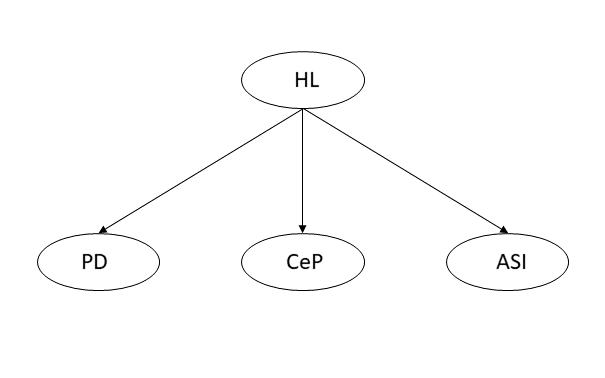
\includegraphics[width=.7\textwidth]{1.png}
	\caption{分级贝叶斯网络模块}
	\label{分级贝叶斯网络模块}
\end{figure}

由于财产损失模块和人员伤亡模块的样本数据具有特征(feature)和标签(label)。因此对于这2个模块,我们采用监督学习的方法来构建,本质上就是找到特征和标签间的映射。对于不良社会影响模块,根据专家知识来构建较为合理。

% Table generated by Excel2LaTeX from sheet 'Sheet1'
\begin{table}[htbp]
	\centering
	\caption{贝叶斯网络结构中的节点变量说明}
	\begin{tabular}{cccp{13.96em}}
		\toprule
		\multicolumn{1}{p{3.575em}}{node ID} & \multicolumn{1}{p{7.075em}}{node name} & \multicolumn{1}{p{4.385em}}{node size} & node value \\
		\midrule
		1     & \multicolumn{1}{p{7.075em}}{date} & 2     & 1=双休日 \\
		&       &       & 0=工作日 \\
		2     & \multicolumn{1}{p{7.075em}}{country} &       & 采用ISO国际标准国家代码 \\
		3     & \multicolumn{1}{p{7.075em}}{region} & 12    & 1=北美 \\
		&       &       & 2=中美洲和加勒比海地区 \\
		&       &       & …… \\
		&       &       & 12=澳大利亚和大洋洲 \\
		4     & \multicolumn{1}{p{7.075em}}{crit1(政治、经济、宗教或社会目标)} & 2     & 1=“是”事件满足标准1 \\
		&       &       & 0=“否”事件不满足标准1或者没有明确表明满足标准1 \\
		5     & \multicolumn{1}{p{7.075em}}{cite2(意图胁迫、恐吓或煽动更多的群众)} & 2     & 1=“是”事件满足标准1 \\
		&       &       & 0=“否”事件不满足标准1或者没有明确表明满足标准1 \\
		6     & \multicolumn{1}{p{7.075em}}{cite3(超出国际人道主义法律范围)} & 2     & 1=“是”事件满足标准1 \\
		&       &       & “否”事件不满足标准1或者没有明确表明满足标准1 \\
		7     & \multicolumn{1}{p{7.075em}}{success(成功的攻击)} & 2     & 1=“是”这一事件是成功的 \\
		&       &       & 0=“否”这一事件不成功的 \\
	
	\end{tabular}%
\label{贝叶斯网络结构中的节点变量说明}%
\end{table}%
	
	\begin{tabular}{cccp{13.96em}}{}
		8     & \multicolumn{1}{p{7.075em}}{suicide(自杀式袭击)} & 2     & 1=“是”这一事件是自杀式袭击 \\
		&       &       & 0=“否”没有任何迹象表明,该事件是一个自杀式袭击 \\
		9     & \multicolumn{1}{p{7.075em}}{attacktype} & 9     & 1=暗杀 \\
		&       &       & 2=武装袭击 \\
		&       &       & …… \\
		&       &       & 9=未知 \\
		10    & \multicolumn{1}{p{7.075em}}{targtype} & 22    & 1=商业 \\
		&       &       & 2=政府(一般意义) \\
		&       &       & …… \\
		&       &       & 22=暴力政党 \\
		11    & \multicolumn{1}{p{7.075em}}{weaptype} & 13    & 1=生物武器 \\
		&       &       & 2=化学武器 \\
		&       &       & …… \\
		&       &       & 13=未知 \\
		12    & \multicolumn{1}{p{7.075em}}{kill(死亡人数)} & \multicolumn{1}{p{4.385em}}{n} & n=死亡总人数减去凶手死亡人数 \\
		13    & \multicolumn{1}{p{7.075em}}{wound( 受伤人数)} & \multicolumn{1}{p{4.385em}}{n} & n=受伤总人数减去凶手受伤人数 \\
		14    & \multicolumn{1}{p{7.075em}}{propexten(财产损害程度)} & 4     & 1=灾难性的 \\
		&       &       & 2=重大的 \\
		&       &       & 3=较小的 \\
		&       &       & 4=未知 \\
		15    & \multicolumn{1}{p{7.075em}}{extended(持续事件)} & 2     & 1=“是”事件的持续时间达到24个小时以上 \\
		&       &       & 0=“否”事件的持续时间不到24小时 \\
		\bottomrule
	\end{tabular}%
	%
\end{table}%

本文先对人员伤亡贝叶斯网络模块的构建进行分析,财产损失的构建方法类似。人员伤亡贝叶斯网络模块中的节点,表示对人员伤亡评估有意义的情报信息或者经过情报机构的专业人员通过数据融合获得的信息。表3表示对于人员伤亡模块,有人员伤亡1个类节点和15个属性节点。

对于本文的人员伤亡模块,其节点变量较少,所以文本用打分搜索方法中的K2算法来构建贝叶斯网络。这个算法需要指定结点的先验顺序。节点顺序主要包括领域知识或节点偏序指定的约束。为了确定唯一的初始节点序,我们首先基于定向后的最大权重跨度树对节点块排序,结点块的排序是唯一的,然后再采用局部完全有向无环图法对块内节点排序,最终得到所有节点的排序结构如图。同理可得财产损失模块的贝叶斯网络结构如图所示。

其次对不良社会影响模块进行分析。根据专家知识可知,恐怖袭击事件造成的不良社会影响跟恐怖袭击事件造成的人员伤亡、财产损失,恐怖主义活动发生前是否威胁、恐吓或向大众传播某种恐怖消息,以及民众或反恐决策人员对恐怖袭击的知情程度密切相关。由此得到图\ref{不良社会影响模块的贝叶斯网络结构}所示的不良社会影响模块的贝叶斯网络结构。TA(terrorist atmosphere)是恐怖份子是否在恐怖活动前对大众造成恐吓或威胁;DK(degree of knowledge)是民众对恐怖袭击的知情程度。PD和TA的状态合集如\ref{不良社会影响模块的贝叶斯网络结构}所示。

\begin{figure}[!h]
	\centering
	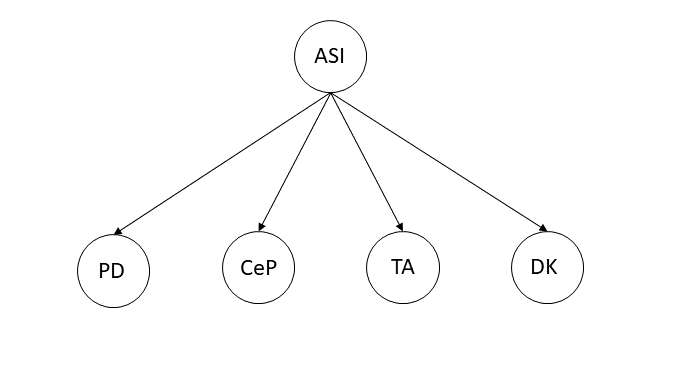
\includegraphics[width=.7\textwidth]{2.png}
	\caption{不良社会影响模块的贝叶斯网络结构}
	\label{不良社会影响模块的贝叶斯网络结构}
\end{figure}

设贝叶斯网络中某一节点$R$,它有$n$个取值,每个取值的先验概率为$p(r_i)$,且$\sum_{i=1}^np(r_i)=1$,节点$R$有一取$m$个值的子节点$S$,$p(S|R)$的条件概率矩阵为
\begin{equation}
	P=\left( \begin{matrix}
	p_{11} & p_{12} & \cdots & p_{1m} \\ 
	p_{21} & p_{22} & \cdots & p_{2m} \\ 
	\vdots & \vdots & \ddots & \vdots \\ 
	p_{n1} & p_{n2} & \cdots & p_{nm}
	\end{matrix} \right).
\end{equation}

财产损失模块和人员伤亡模块贝叶斯网络,由于存在观测数据,可以从数据中学习参数的概率分布表,但没有与分级贝叶斯网络和不良社会影响模块贝叶斯网络相关的观测数据,所以这2个贝叶斯网络模块的概率分布表采用主观赋权法来确定。
考虑多个专家给出$p(S|R)$的条件概率矩阵为
\begin{equation}
P^k=\left( \begin{matrix}
p_{11} & p_{12} & \cdots & p_{1m} \\ 
p_{21} & p_{22} & \cdots & p_{2m} \\ 
\vdots & \vdots & \ddots & \vdots \\ 
p_{n1} & p_{n2} & \cdots & p_{nm}
\end{matrix} \right).
\end{equation}

其中$k=1,2,\cdots,q$表示专家的个数,设每个专家的权重为$H=(h_1,h_2,\cdots,h_q)^T$,其中$\sum_{k=1}^qh_k=1$.为了确定各条件概率值,建立优化模型:
%谁来搞一下这个公式
	\begin{equation} \label{eqn3}
\begin{center}
$$\min L=\sum\limits_{i=1}^{n}p(a_i) \sum\limits_{k=1}^{q}\sum\limits_{j=1}^{m}h_k(p_{ij}- p_{ij}^k)^2 $$

$$\mathrm{s.t.}\sum\limits_{j=1}^{m}p_{ij}=1(i=1,2,\cdots,n)$$

$$	p_{ij}\geq 0(i=1,2,\cdots,n;j=1,2,\cdots,m)$$
\end{center}

\end{equation}


该优化模型的目标是使条件概率矩阵与专家给出的条件概率之间的总偏差平方和最小。由$\frac{\partial L}{\partial p_{ij}}$得条件概率的主观概率为
\begin{equation}
	p_{ij}=\sum_{k=1}^{q}h_kp_{ij}^k(i=1,2,\cdots,n;j=1,2,\cdots,m).
\end{equation}
\subsection{问题求解}
多模块贝叶斯网络的实现:根据上文中提出的多模块贝叶斯网络,可以从观测到的事件出发,逐层推理,得到置换节点的状态,最后再由置换节点的状态推理得到恐怖袭击的危害性分级。由于它是多模块集成的,不同模块的贝叶斯网络结构差异较大,所以针对不同的模块,选择不同的推理算法。对于分级贝叶斯网络模块,贝叶斯网络中不含有回路,本文采用Pearl提出的多树传播推理算法;其他3个贝叶斯网络模块采用联结树推理算法。

本文先将贝叶斯网络转化为联结树,然后对联结树上的消息传递过程进行定义,再计算概率,基本过程如下:
1、建立Moral图:将有向图转换为无向图,找出每个节点的父节点并连接起来把所有的有向边改为无向边

2、将Moral图三角化:三角化是指让图中不存在超过3个点的环。将大于等于4的环,取其中两个非相邻节点用无向边连接起来,进行Moral图的三角化,即对顶点的一一删除。具体规则为(1)成对的联结该顶点的相邻节点;(2)删除该节点,并添加边;(3)删除的顶点必须保证,所需要添加的边最少。

3、在三角化的图中确定团:每个三角都代表了一个节点,两个相临的三角具有共同的边。这条边就成为两个节点之间的中间节点。如此就组成一张联通图。找到三角化后Moral图中构成联结树的所有团,团即为最大全联通子图,其中每对不同节点都有边相连。

4.建立联结树

根据已获得的关于恐怖袭击事件的证据信息$[X_1,X_2,\cdots,X_n]$,用联结树传播算法推理得到财产损失模块和人员伤亡模块的后验概率,然后根据这两个后验概率用消息传递算法推理得到不良社会影响的后验概率,最后,用子模块的结果得到分级贝叶斯网络中恐怖袭击危害性等级的后验概率,算法的过程如下:
\IncMargin{1em} % 使得行号不向外突出 
\begin{algorithm}
	
	\SetAlgoNoLine % 不要算法中的竖线
	\SetKwInOut{Input}{\textbf{输入}}\SetKwInOut{Output}{\textbf{输出}} % 替换关键词
	
	\Input{
		\\
		证据$[X_1,X_2,\cdots,X_n]$,多模块贝叶斯网络\;\\
	}
	\Output{
		\\
		根节点恐怖袭击危害性等级HL的置信度\;\\
	}
	\BlankLine
	
	根据部分证据[$[X_1,X_2,\cdots,X_i](i<n)$ ,对人员伤亡和财产损失模块的贝叶斯网络,调用联结树传播算法计算得到财产损失节点PD和人员伤亡节点CeP的后验概率\; % 分号 \; 区分一行结束
	用PD和CeP后验概率以及证据$[X_j,X_j+1,\cdots,X_n](i<j<=n)$,对不良社会影响模块的贝叶斯网络调用联接树传播算法得到不良社会影响节点ASI的后验概率\;
	对分级贝叶斯网络模块,确定根节点恐怖袭击危害性HL的先验信息,并初始化根节点HL的置信度Bel(HL),令$Bel(HL) = π(HL)$\;
	\Repeat
	{\text{后验概率=先验概率,返回根节点HL}}
	{对分级贝叶斯网络模块,若某一子节点$\theta$的诊断信息发生变化,变化为$\lambda_\theta$,则根节点HL的诊断信息变化为$λHL = M_\theta × \lambda_\theta$, 其中$M_\theta$为 某一子节点关于根节点的条件概率矩阵\;
		向上更新根节点HL的置信值,更新后根节点HL的置信度为$Bel(HL) = \partial × (\lambda_{HL}· π(HL))$。其中“·”为内积算子, $\partial$为归一化因子,其作用是使根节点HL不同状态的置信度的和为1\;
		向下更新子节点$\theta$的置信度,更新后子节点$\theta$的置信度为$Bel(\theta) = \partial × {M_\theta}^T × Bel(HL)$\;
		
	}
	\caption{多模块贝叶斯网络\label{al1}}
\end{algorithm}
\DecMargin{1em}

最后得到结果如表\ref{die},\ref{die2}
\begin{table}[htbp]
	\centering
	\caption{危害程度最高的十大恐怖袭击事件}
	\begin{tabular}{ccc}
		\toprule
		Number & Eventid & Country \\
		\midrule
		1     & 200109110004 & United States \\
		2     & 200409010002 & Russia \\
		3     & 201101240016 & Russia \\
		4     & 201403010012 & China \\
		5     & 200507070001 & United Kingdom \\
		6     & 201304150001 & United States \\
		7     & 201107220012 & Norway \\
		8     & 200811260001 & India \\
		9     & 200412030001 & Spain \\
		10    & 201004040002 & Russia \\
		\bottomrule
	\end{tabular}%
	\label{die}%
\end{table}%
\begin{table}[htbp]
	\centering
	\caption{典型事件危害级别}
	\begin{tabular}{cc}
		\toprule
		事件编号  & 危害级别 \\
		\midrule
		200108110012 & 1 \\
		%\midrule
		200511180002 & 4 \\
		%	\midrule
		200901170021 & 1 \\
		%\midrule
		201402110015 & 5 \\
		%	\midrule
		201405010071 & 4 \\
		%	\midrule
		201411070002 & 3 \\
		%	\midrule
		201412160041 & 2 \\
		%	\midrule
		201508010015 & 3 \\
		%	\midrule
		201705080012 & 4 \\
		\bottomrule
	\end{tabular}%
	\label{die2}%
\end{table}%

\section{问题二}
\subsection{问题分析}
本文的恐怖袭击事件中人员伤亡和参与人数、攻击方式和财产损失等关系也是相对固定的。在同一领域的模型中,案例之间的相似程度可以近似的通过计算相同节点的数目获得,就是说两个节点相似程度高的模型,它们的网络结构也具有很高的相似度。这就需要利用案例适配的方法,案例适配的主要思想就是利用历史案例与新案例的相似程度,以相似程度最大的案例作为匹配结果。灰色系统理论为我们提供了崭新的多因素分析方法—灰色关联分析方法。灰色关联是指事物间的不确定关联,或系统因子之间、因子对主行为之间的不确定关联。灰色关联分析是一种用灰色关联度顺序(简称为灰关联序)来描述因素间关系的强弱、大小、次序的方法,是通过灰色关联度来分析和确定系统因素间的影响程度或因素对系统主行为的贡献测度的一种方法。其基本思想是:以因素的数据序列为依据,用数学的方法研究因素间的几何对应关系,即序列曲线的几何形状越接近,则它们之间的灰关联度越大,反之越小。

\subsection{模型建立}
设系统特征行为序列(子节点或类节点序列)为
\begin{equation}
	X_0(k)=(x_0(1),x_0(2),\cdots,x_0(n))
\end{equation}

系统的相关因素行为序列为
\begin{equation}
	X_i(k)=(x_i(1),x_i(2),\cdots,x_i(n)),(i=1,2,\cdots,m)
\end{equation}

本文采用计算$X_0$和$X_i$的B型关联度模型。

首先计算关联系数为:
\begin{equation}
\gamma(X_0,X_i)=\frac{1}{1+\frac{1}{n}d_{0i}^{(0)}+\frac{1}{n-1}d_{0i}^{(1)}+\frac{1}{n-2}d_{0i}^{(2)}}
\end{equation}
其中:
\begin{equation}
	d_{0i}^{(0)}=\sum_{k=1}^{max}d_{0i}^{(0)}(k)=\sum_{k=1}^{n}|x_0(k)-x_i(k)|
\end{equation}
\begin{equation}
	d^{(1)}_{0i}=\sum_{k=1}^{n-1}d_{0i}^{(1)}(k)=\sum_{k=1}^{n-1}|x_0(k+1)-x_i(k+1)-x_0(k)+x_i(k)|
\end{equation}
\begin{equation}
	d^{(2)}_{0i}=\sum_{k=2}^{n-1}d_{0i}^{(1)}(k)=\frac{1}{2}\sum_{k=2}^{n-1}|[x_0(k+1)-x_i(k+1)]-2[x_0(k)-x_i(k)]+[x_0(k-1)0-x_i(k-1)]|
\end{equation}

$d_{0i}^{(0)}$,$d_{0i}^{(1)}$,$d_{0i}^{(2)}$分别为离散函数$x_0(k)$与$x_i(k)$的位移差、一阶斜率差、二阶斜率差。
\section{问题三}
本文采用向量自回归模型、脉冲响应函数和方差分解研究方法对恐怖袭击事件内生性进行研究。VAR模型是一种基于数据的统计性质的非结构化模型,它把系统中每一个内生变量作为系统中所有内生变量的滞后值来构造模型,从而将单变量自回归模型推广到多元时间序列变量组成的向量自回归模型。VAR($p$)模型数学表达式为:
\begin{equation}
	y_t=a_1y_{t-1}+a_2y_{t-2}+\cdots+a_py_{t-p}+bx_t+\varepsilon_t,t=1,2,\cdots,T
\end{equation}

其中,$y_t$是k维内生向量组成的平稳的线性随机过程,$x_t$是$d$维外生向量,$p$是滞后阶数,$T$是样本个数,$k*k$维矩阵$a_1,a_2$,$\cdots$,$a_p$和和$k*‘d$维矩阵$b$是待估计的系数矩阵。$\varepsilon_t$是k维扰动误差项,它们相互之间可以同期相关,但不与自己的滞后值相关,且不与等式右边的变量相关,即假设$\sum$是$\varepsilon_t$的协方差矩阵,是一个$kxk$正定矩阵。

在VAR模型中,可以通过脉冲响应函数可以分析恐怖袭击行为与时间、地域分布,事件相关性等因素。方差分解分析法把系统中的全部内生变量(m个)的波动按其成因分解为与各个方程信息相关联的m个组成部分。在本文中,通过方差分解可以确定恐怖袭击事件发生的主要原因、时空特性、蔓延特性、级别分布等规律。

\subsection{变量选取}
本文分析近三年来的恐怖袭击事件,基于数据连续性和可获得性,选取的变量如下:

(1)事件发生的原因。恐怖分子袭击定义有三个标准:标准1:暴力行为旨在实现政治、经济、宗教和社会性目标;标准2:具有一些证明暴力行为意图胁迫、恐吓或向更多的读者传达一些信息的证据;标准3:该行动必须是在合法战争活动的背景下进行的。假设以此标准作为恐怖袭击发生的原因。

(2)事件发生的时间、地点。恐怖袭击的时间和地域、城市等信息均在附件一中给出。

(3)事件的相关性。在问题二中,我们已经通过灰色预测得出了部分恐怖袭击事件的关联程度。

(4)事件的级别分布。问题一中,我们使用多模块的贝叶斯网络对恐怖袭击进行了分级。

\subsection{模型求解}
通过脉冲响应函数可以分析恐怖袭击发生的主要原因、时空特性、蔓延特性、级别分布等规律。方差分解分析法把系统中的全部内生变量(m个)波动按其成因分解为与各个方程信息相关联的m个组成部分。通过方差贡献度的大小,可以衡量随机扰动项对各变量的相对重要程度。在本文中,通过方差分解可以确定主要原因、时空特性、蔓延特性、级别分布对恐怖袭击的影响,进而预测下一年全球的恐怖袭击发展态势。因此需要对序列进行平稳性检验。若序列平稳,则构造回归模型;若序列非平稳,需对原序列进行差分,直到第i阶平稳。在序列平稳的基础上,构造VAR模型,进而进行脉冲响应函数和方差分解分析。
\subsection{对反恐战争的见解和建议}
恐怖分子作案前,一般都会流露出异常迹象,也会在金钱、作案工具、作案人员等方面进行准备或串联,如果能收集掌握一个个看似微不足道的异常信息,进行整合分析,就能形成灵敏的预警机制,制敌于未动,将
恐怖袭击消灭在发生之前。“9·11”事件后,恐怖主义在全球呈蔓延态势,在此后的十多年内成为威胁国家安全和地区稳定的重要因素。近年来,以“伊斯兰国”异军突起为标志,国际恐怖主义正在掀起新的一轮浪潮,呈现出不同于以往的新态势。面对日益严峻的国际反恐斗争,本文通过对国际恐怖主义的现状进行统计分析,探究当前全球恐怖主义活动的发展特点,预测未来国际恐怖主义的变化趋势,从而得出新形势下国际恐怖主义给世界各国带来的挑战,探究世界反恐怖工作应当作出的应对之策,从而为保护世界人民安全和利益、维护全球秩序和稳定迈出坚实的一步。全球恐怖主义的新态势对海外安全与利益、全球反恐怖斗争工作与促进世界繁荣与发展等方面带来了新挑战,应通过以总体安全观为指导、以联合国反恐怖法案条例为依据、以情报建设为抓手,统筹国际反恐国际,并以反恐专业力量为依托,准确把握国际恐怖活动发展趋势,提前谋划应对之策,破解越反越恐的现实困境。
\section{问题四}
	\subsection{问题分析}
前文给出的贝叶斯网络例子中,每一个节点(随机变量)都有唯一的一个固定取值。当我们观察一个结果或状态时(例如恐怖袭击发生的概率),我们的任务是据此推断发生恐怖袭击地区的人均生产总值。而在此过程中,恐怖袭击是否发生并不会改变,而人均生产总值也不会改变。这就说明,我们其实是在一个静态的世界中来进行推理的。而隐马尔科夫模型(Hidden Markov Model,HMM)就是解决这类问题时最常用的一种数学模型。
\subsection{模型建立}
给定一个时间序列观测$O=O_1O_2\cdots O_T$和HMM模型$\lambda=(A,B.\pi)$,一个直接计算$p(O|\lambda)$的方法是遍历所有可能的状态路径,并把它们产生的概率相加,如下式:
\begin{equation}
P(O|\lambda)=\sum_{Q}P(O,Q|\lambda)=\sum_{Q}b_{q1}(O_1)b_{q2}(O_2)\cdots b_{qT}(O_T) \pi_{q1}a_{q1q2}a{q2q3}\cdots a_{qT-1qT}
\end{equation}
\newpage

%参考文献   手工录入
%\begin{thebibliography}{9}%宽度9
% \bibitem{bib:one} ....
% \bibitem{bib:two} ....
%\end{thebibliography}
\begin{thebibliography}{123456}
	\bibitem {1}P. Elzinga, J. Poelmans, S. Viaene, G. Dedene and S. Morsing, "Terrorist threat assessment with formal concept analysis," 2010 IEEE International Conference on Intelligence and Security Informatics, Vancouver, BC, 2010, pp. 77-82.
	\bibitem {2} S. Navid Shahrouzi, Darshika G. Perera. Dynamic partial reconfigurable hardware architecture for principal component analysis on mobile and embedded devices. S. Navid Shahrouzi, Darshika G. Perera. EURASIP Journal on Embedded Systems, 2017, Volume 2017, Number 1, Page 1
	\bibitem {3} J. Allanach, Haiying Tu, S. Singh, P. Willett and K. Pattipati, "Detecting, tracking, and counteracting terrorist networks via hidden Markov models," 2004 IEEE Aerospace Conference Proceedings (IEEE Cat. No.04TH8720), Big Sky, MT, 2004, pp. 3246-3257 Vol.5.
	\bibitem {4} Xiaoquan Tang,Long Zhang,Xiuting Li. Bayesian augmented Lagrangian algorithm for system identification[J]. Systems and Control Letters,2018,120.
	\bibitem {5}邹晓辉.朴素贝叶斯算法在文本分类中的应用[J].数字技术与应用,2017(12):132-133.
	\bibitem {6}王双成. 贝叶斯网络学习、推理与应用. [M]. 上海:立信会计出版社. 2010.
	\bibitem {7}马骞. 聚类算法概述与应用.[J]. 中国新通信.2018,20(14):225-226.
	\bibitem {8}张伦干. 多项式朴素贝叶斯文本分类算法改进研究[D].中国地质大学,2018.
	\bibitem {9}徐保鑫,怀丽波. 基于MapReduce的朴素贝叶斯算法在新闻分类中的应用[J].延边大学学报(自然科学版),2017,43(01):55-59.
	\bibitem {10}赵文涛,孟令军,赵好好,韩炳权,成亚飞.分布式朴素贝叶斯算法在文本分类中的应用[J].测控技术,2016,35(06):50-55.
	\bibitem {11}严嘉铭,黄理灿.基于MapReduce	的朴素贝叶斯文本分类研究[J].工业控制计算机,2016,29(04):96-97.
	\bibitem {12}张佳.计算机数据挖掘技术的开发及其应用[J/OL].电子技术与软件工程,2018(17):172-173[2018-09-18]. 
	\bibitem {13}张凯萍.大数据时代背景下数据挖掘技术的应用探讨[J].赤峰学院学报(自然科学版),2018,34(08):52-54.
	\bibitem {14}於冉,黄天齐,於忠祥.基于主成分分析的安徽省城市层级划分研究[J/OL].安徽农业大学学报:1-7[2018-09-18].
	\bibitem {15}张冰怡.当代世界恐怖主义及其全球治理对策——基于2017年以来欧美多次恐怖袭击的思考[J].南方论刊,2018(05):16-18+21.
	\bibitem {16}王奇,田一鸣.全球恐怖活动的GTD数据分析与我国应对之策[J].犯罪研究,2018(02):87-96.
	\bibitem {17}李益斌.欧洲恐怖主义的新态势及原因分析——基于聚类分析法[J].情报杂志,2018,37(03):55-63.
	\bibitem {18}陈杰,邬春学.决策树C4.5算法改进与应用[J/OL].2018(09):1-5.
	
\end{thebibliography}	
%采用bibtex方案

%\cite{mittelbach_latex_2004,wright_latex3_2009,beeton_unicode_2008,vieth_experiences_2009}
%\bibliography{example}

\newpage
%附录
\appendix
%\setcounter{page}{1} %如果需要可以自行重置页码。
\section{我的 Python 源程序}
\begin{lstlisting}[language=Python]%设置不同语言即可。
import xlrd
import numpy as np
def isLUN(year):
if year%100==0:
if year%400==0:
return 1
else:
if year%4==0:
return 1
return 0

def dijitian(YEAR,Month,day):
ret=0
ping=[31,28,31,30,31,30,31,31,30,31,30,31]
lun=[31,29,31,30,31,30,31,31,30,31,30,31]
if isLUN(YEAR):
for i in range(Month-1):
ret=ret+lun[i]
else:
for i in range(Month-1):
ret=ret+ping[i]
return ret+day;



def jiejiari(YEAR,Month,day):
S=(YEAR+(YEAR-1)//4-(YEAR-1)//100+(YEAR-1)//400)%7
days=(dijitian(YEAR,Month,day)+S-1)%7
#return days
if days==0 or days==6:
return 1
else :
return 0

fname = 'data1.xlsx'
bk = xlrd.open_workbook(fname)
shxrange = range(bk.nsheets)
try:
sh = bk.sheet_by_name('Data')
except:
print('no sheet in %s named Data',format(fname))

nrows = sh.nrows
ncols = sh.ncols
print('nrows: {0},ncols: {1}'.format(nrows,ncols))
#获取第一行第一列
cell_value = sh.cell_value(1,1)
row_list = []
col_list = []
#print(cell_value)
#获取各行数据
#for i in range(0,nrows):
#row_data = sh.row_values(i)
#row_list.append(row_data)
#print(row_list)

#获取各列数据
x = np.array(sh.col_values(0))
for i in range(1,ncols):
col_data = sh.col_values(i)
x = np.c_[x,np.array(col_data)]
#col_list.append(col_data)

year = x[1:,1]
month = x[1:,2]
day = x[1:,3]

weekday = []
for j in range(0,nrows-1):
w = jiejiari(round(float(year[j])),
round(float(month[j])),round(float(day[j])))
weekday.append(w)

print(len(weekday))
#print(weekday)

#symbol = Symbol(col_list[0],col_list[1],col_list[2],col_list[3])
#print(symbol.eventid[0])
#print(col_list)
print(jiejiari(2018,9,16))

import numpy as np
import matplotlib.pyplot as plt

from sklearn.datasets import load_iris
from sklearn.decomposition import PCA, IncrementalPCA

iris = load_iris()
X = iris.data
y = iris.target

n_components = 2
ipca = IncrementalPCA(n_components=n_components, batch_size=10)
X_ipca = ipca.fit_transform(X)

pca = PCA(n_components=n_components)
X_pca = pca.fit_transform(X)

colors = ['navy', 'turquoise', 'darkorange']

for X_transformed, title in [(X_ipca, "Incremental PCA"), (X_pca, "PCA")]:
plt.figure(figsize=(8, 8))
for color, i, target_name in zip(colors, [0, 1, 2], iris.target_names):
plt.scatter(X_transformed[y == i, 0], X_transformed[y == i, 1],
color=color, lw=2, label=target_name)

if "Incremental" in title:
err = np.abs(np.abs(X_pca) - np.abs(X_ipca)).mean()
plt.title(title + " of iris dataset\nMean absolute unsigned error "
"%.6f" % err)
else:
plt.title(title + " of iris dataset")
plt.legend(loc="best", shadow=False, scatterpoints=1)
plt.axis([-4, 4, -1.5, 1.5])

plt.show()
 \end{lstlisting}


\end{document} 